\chapter{Existing Methods}

% Chapter Introduction
Three-dimensional reconstruction from two-dimensional images has been an active area of research in computer vision for many years. Several techniques have been developed to generate 3D structures from image data, each with its own advantages and limitations. Most existing methods focus on achieving high accuracy and detailed reconstruction, often relying on computationally intensive algorithms or deep learning models.

Traditional approaches such as Structure from Motion (SfM) and Multi-View Stereo (MVS) use multiple images captured from different viewpoints to estimate camera positions and reconstruct the 3D structure of a scene. These methods are widely used due to their accuracy, but they require significant processing power and are not suitable for real-time or mobile-based applications.

Recent advancements in deep learning have introduced monocular depth estimation models that can predict depth from a single image. Models such as MiDaS and ZoeDepth have shown promising results in generating dense depth maps. However, these models are typically large and require optimization before they can be deployed efficiently on mobile devices. \\ \\

In addition to these methods, sensor-based approaches using depth cameras such as LiDAR and structured light have also been explored. These systems provide accurate depth information but require specialized hardware, which increases the cost and limits accessibility for general users. As a result, purely vision-based methods remain an attractive solution for mobile applications. \\ \\

% Section 1
\section{Cloud-Based Reconstruction Systems}

Another widely used approach is cloud-based 3D reconstruction. In this method, images captured from a device are uploaded to remote servers where powerful GPUs process the data and generate a 3D model. This approach produces high-quality results and supports complex reconstruction tasks.

However, cloud-based solutions introduce several challenges. They depend on stable internet connectivity, which may not always be available. Additionally, sending image data to external servers raises privacy concerns and increases latency. These limitations make such systems less practical for real-time and offline applications.

Some mobile-based solutions have also been proposed to perform reconstruction directly on smartphones. These systems aim to reduce dependency on external resources but often compromise on accuracy or processing speed. Many of them do not fully utilize modern deep learning techniques, limiting their performance. \\ \\

Another drawback of cloud-based systems is scalability. As the number of users increases, the demand for server resources also grows, leading to higher operational costs. Furthermore, large-scale data transfer can result in bandwidth limitations, especially in regions with poor network infrastructure. These issues further highlight the need for efficient on-device solutions.

% Section 2
\section{3D Reconstruction Pipeline}

A typical 3D reconstruction pipeline consists of multiple stages, including image acquisition, feature extraction, camera pose estimation, depth estimation, and mesh generation. Feature matching techniques are used to identify correspondences between images, which helps in estimating camera motion.

Depth maps obtained from sensors or neural networks are combined using fusion techniques to create a unified 3D representation. Finally, surface reconstruction algorithms generate a mesh that represents the object or scene. While this pipeline is effective, it is computationally expensive and difficult to execute efficiently on low-power mobile devices.

Each stage of the pipeline introduces its own set of challenges. For instance, feature extraction must be robust to variations in lighting and viewpoint. Camera pose estimation requires accurate matching of features across frames, which can be affected by noise or motion blur. Depth estimation models must balance accuracy and computational efficiency, especially when deployed on mobile hardware.

Moreover, mesh generation and visualization require efficient data structures and rendering techniques to ensure smooth performance. Without proper optimization, these processes can lead to high memory consumption and reduced frame rates, affecting the overall user experience.

% Figure
\begin{figure}[H]
    \centering
    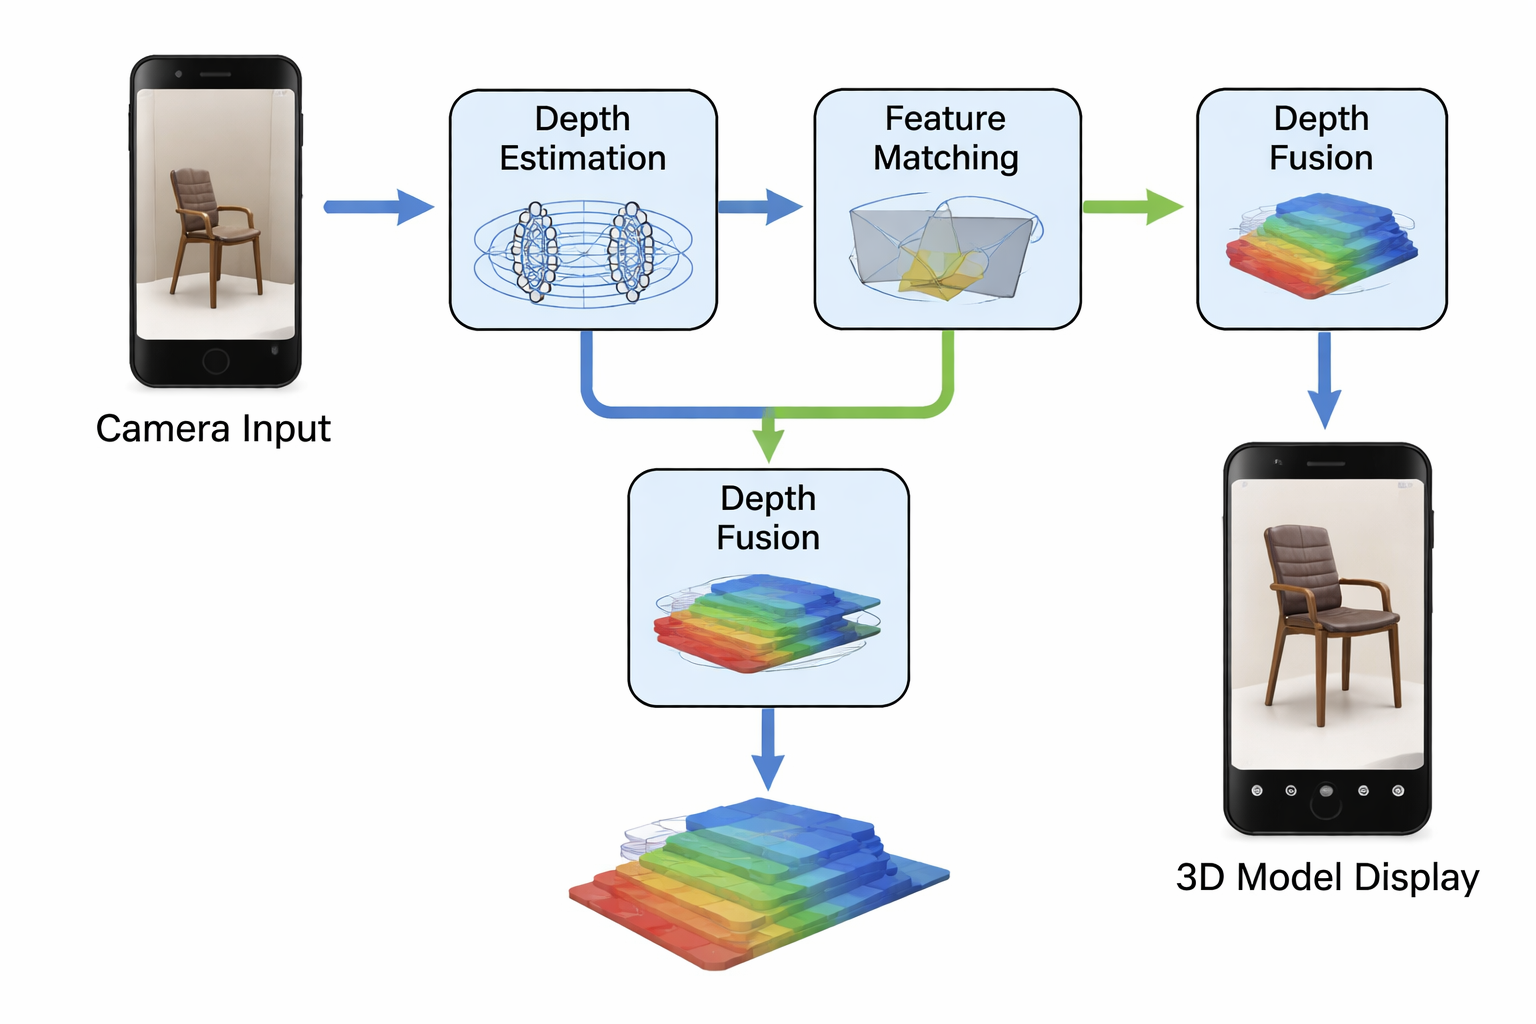
\includegraphics[width=400pt]{Images/subsection2.png}
    \caption{Block diagram of the device}
\end{figure}

% Conclusion
From the analysis of existing methods, it is clear that there is a trade-off between accuracy and efficiency. High-quality reconstruction systems require powerful hardware or cloud support, while lightweight solutions struggle to maintain accuracy. This highlights the need for a balanced approach that can deliver acceptable performance while remaining efficient and portable. \\ \\

Furthermore, the integration of deep learning with traditional geometric methods has opened new possibilities, but also introduced additional computational challenges. Optimizing these hybrid approaches for mobile environments remains an important area of research.

\newpage

% Section 3
\section{Motivation}

The limitations of existing systems highlight the need for a more practical solution that can operate entirely on mobile devices. With the increasing demand for applications such as augmented reality, mobile scanning, and offline visualization, it is important to develop systems that are both efficient and independent of internet connectivity.

This project is motivated by the goal of enabling 3D reconstruction directly on ARM-based mobile devices without relying on external computation. By combining lightweight deep learning models with optimized geometric processing techniques, the proposed system aims to achieve a balance between performance, accuracy, and usability in real-world scenarios.

In addition, the growing availability of smartphones with improved processing capabilities provides an opportunity to shift complex computations from cloud environments to edge devices. This transition not only enhances privacy but also reduces dependency on external infrastructure.

The motivation also stems from the need to make 3D reconstruction technology more accessible to a wider audience. By eliminating the requirement for specialized hardware or high-end systems, the proposed solution enables everyday users to generate 3D content easily using their mobile devices.

Finally, this work aims to contribute toward the development of efficient and scalable mobile vision systems, paving the way for future innovations in areas such as real-time augmented reality, digital twin creation, and intelligent mobile sensing.